% The proposed method, one outer iteration, with what each step costs and
% whether it is independent per courier.  Greyscale, for print.
%
%   pdflatex fig_pipeline.tex
%
% Laid out narrow, so that it stays legible at one IEEE column width.
% Times are measured at |R| = 1000, |K| = 300, Q_k = 5, phi = 100.

\documentclass[border=4pt]{standalone}
% the same Charter face as the manuscript body, so the schematic
% does not read as a different document
\usepackage{XCharter}
\usepackage{tikz}
\usepackage{booktabs}
\usetikzlibrary{arrows.meta,positioning,fit,backgrounds,calc}

\begin{document}

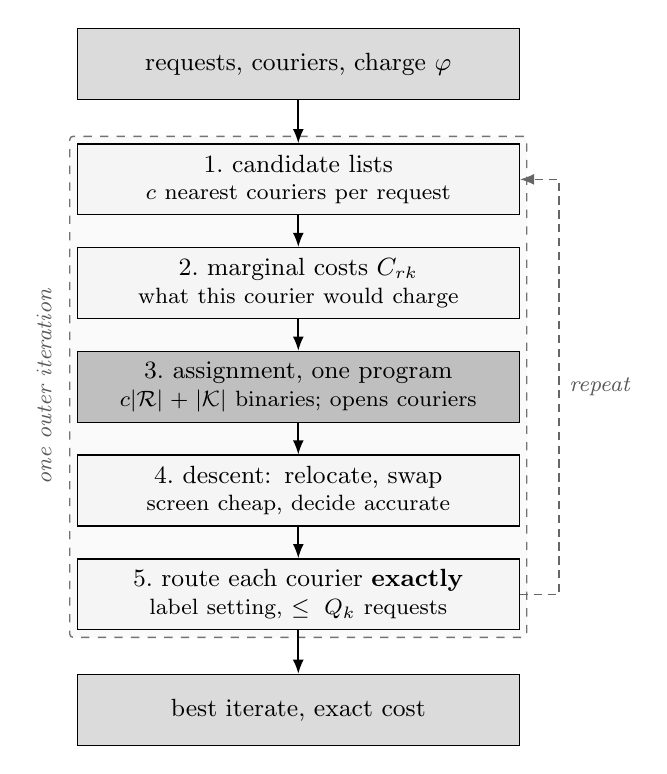
\begin{tikzpicture}[
  font=\small,
  >={Latex[length=1.8mm,width=1.4mm]},
  box/.style   = {draw=black, line width=0.5pt, fill=white, align=center,
                  inner sep=3pt, minimum height=9mm, text width=54mm},
  io/.style    = {box, fill=black!14},
  par/.style   = {box, fill=black!4},
  ser/.style   = {box, fill=black!25},
  loop/.style  = {draw=black!55, line width=0.5pt, dashed,
                  rounded corners=1.2pt, fill=black!2},
  arr/.style   = {->, line width=0.6pt}
]

\node[io]  (in)  at (0,0)              {requests, couriers, charge $\varphi$};
\node[par] (c1)  [below=5.5mm of in]   {1.\ candidate lists\\[-1pt]
                                        \footnotesize $c$ nearest couriers per
                                        request};
\node[par] (c2)  [below=4mm of c1]     {2.\ marginal costs $C_{rk}$\\[-1pt]
                                        \footnotesize what this courier would
                                        charge};
\node[ser] (c3)  [below=4mm of c2]     {3.\ assignment, one program\\[-1pt]
                                        \footnotesize $c|\mathcal{R}|+|\mathcal{K}|$
                                        binaries; opens couriers};
\node[par] (c4)  [below=4mm of c3]     {4.\ descent: relocate, swap\\[-1pt]
                                        \footnotesize screen cheap, decide
                                        accurate};
% Not "<= 8 requests": 8 is where our implementation stops running the exact
% router, not a property of the method, and it never binds -- capacity holds
% a courier's set to Q_k, which is 5 throughout the experiments.
\node[par] (c5)  [below=4mm of c4]     {5.\ route each courier
                                        \textbf{exactly}\\[-1pt]
                                        \footnotesize label setting, $\le Q_k$
                                        requests};
\node[io]  (out) [below=5.5mm of c5]   {best iterate, exact cost};

\begin{scope}[on background layer]
  \node[loop, fit=(c1)(c5), inner sep=2.5pt] (L) {};
\end{scope}
% The dashed region is the outer iteration.  Unlabelled it reads as
% decoration, and the caption's "one outer iteration" then looks like it
% describes the whole diagram, input and output boxes included.
\node[rotate=90, anchor=south, font=\footnotesize\itshape, text=black!65]
  at ([xshift=-1.0mm]L.west) {one outer iteration};

\draw[arr] (in)--(c1); \draw[arr] (c1)--(c2); \draw[arr] (c2)--(c3);
\draw[arr] (c3)--(c4); \draw[arr] (c4)--(c5); \draw[arr] (c5)--(out);
\draw[->, line width=0.6pt, densely dashed, draw=black!60]
  (c5.east) -- ++(5mm,0) |- (c1.east)
  node[pos=0.25, right, font=\footnotesize\itshape, text=black!65]
  {repeat};

% The measured per-step timings used to hang below this diagram as a strip.
% They were moved to Section V's scaling discussion, which is the first place
% the instance, the machine and the design rule behind them are defined; here
% in the method overview they arrived before any of that, and every number in
% them already appears in that section and its table.

\end{tikzpicture}

\end{document}
